\section{System Architecture and Implementation}

\subsection{From Specification to Running System}

SIDS 2026 \cite{katrakazas2026} proposed a three-tier architecture for participatory data sovereignty: a Mobile Application Layer where consent is captured at the interface, a Synchronization Layer where a device-side filter enforces what leaves the device, and a Backend Services Layer where a community steward model gates what is released beyond the device tier. That paper's own "Technical Implementation Status" section was explicit about what stood behind each claim: the mobile application, local storage with offline queuing, and the CouchDB backend with a k-anonymity pipeline were functional, while the differential-privacy mechanisms, privacy-budget tracking, and the steward portal itself were, in its own words, still in the design and specification phase pending pilot deployment. The steward quorum gate that paper described, an aggregated output wrapped in an envelope keyed by steward quorum with the decryption key released only on receipt of a co-signed authorization token, existed as a written design, not as code that had been built and run.

This chapter reports what has since actually been built to realize that architecture, following the same three-layer structure SIDS 2026 introduced, but now describing running software rather than a specification. It also reports, honestly, where the built system diverges from the design as originally written: the steward-release cryptographic envelope did not survive into the implementation in the form SIDS 2026 described, the single-steward veto that same paper specified as part of the release gate is recorded but not enforced by the built system, and the connector's audit coverage turned out to have a boundary that the original design did not anticipate. All three corrections are load-bearing for what this paper can claim, and each is documented in the project's own design record, rather than being retrofitted here.

The reference implementation lives in a single repository organized around the same three tiers. A TypeScript workspace (\texttt{packages/}) implements the consent model and its two compilation targets, plus participant-side audit verification and a simulated device fleet. Two browser applications (\texttt{apps/participant-web}, \texttt{apps/steward-portal}) and one Flutter mobile application (\texttt{apps/participant-mobile}) provide the interface layer. A Java connector (\texttt{connector/}), built on Eclipse Dataspace Components (EDC) and organized into three extensions, \texttt{benefits-policy}, \texttt{benefits-privacy}, and \texttt{benefits-audit}, implements the release boundary. The remainder of this chapter walks the built system tier by tier, positioning each subsystem against the closest work identified in the literature search that grounds this paper's Related Work chapter.

\begin{figure}[H]
\centering
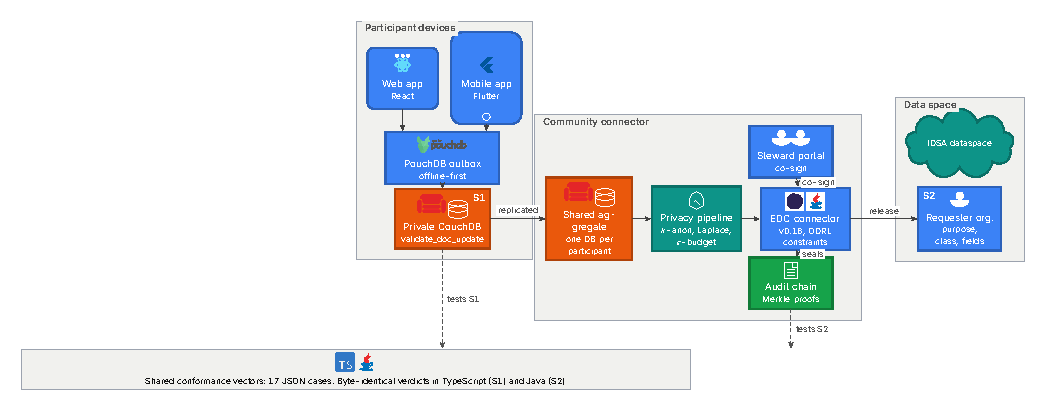
\includegraphics[width=\linewidth, totalheight=0.95\textheight, keepaspectratio]{../figures/schematics/fig-system-architecture.pdf}
\caption{The full system architecture, tier by tier, from participant devices through the community connector to the data space.}
\label{fig:architecture}
\end{figure}

\begin{figure}[H]
\centering
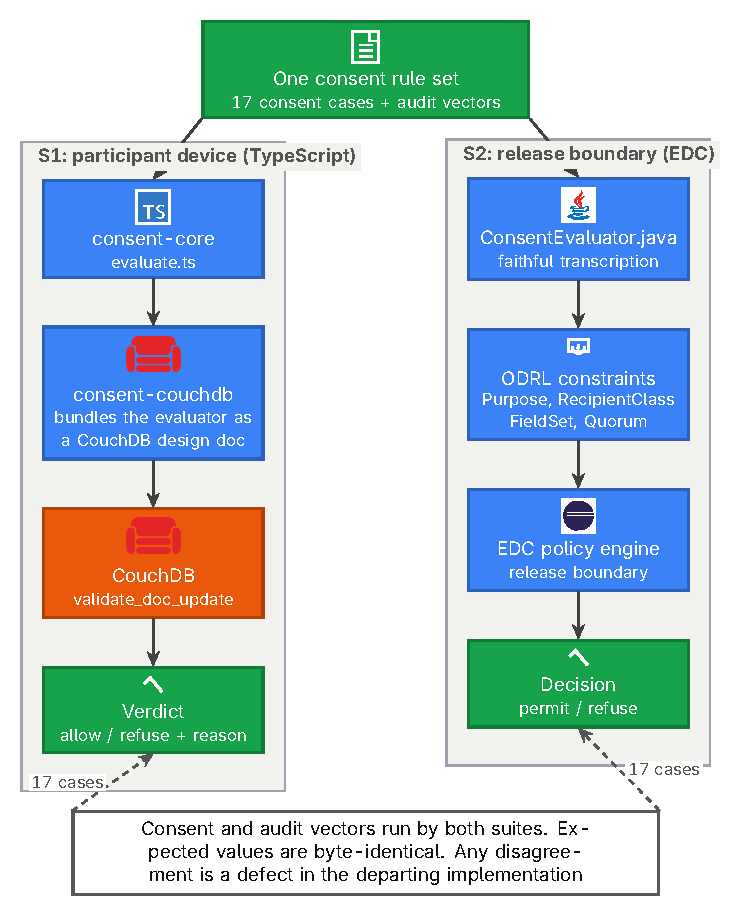
\includegraphics[width=\linewidth, totalheight=0.85\textheight, keepaspectratio]{../figures/schematics/fig-enforcement-points.pdf}
\caption{The two enforcement points, the CouchDB validator at the device boundary and the EDC constraint functions at the connector boundary, pinned together by the shared conformance vectors.}
\label{fig:enforcement-points}
\end{figure}

\begin{figure}[H]
\centering
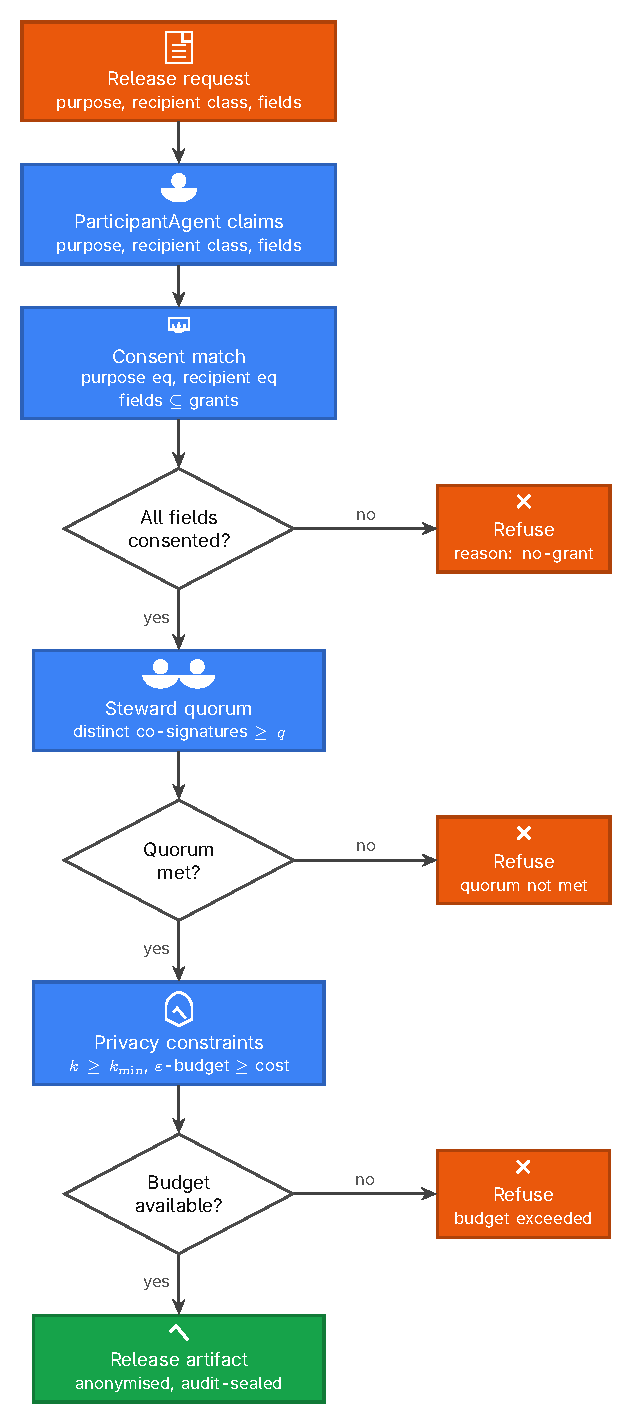
\includegraphics[height=0.85\textheight, keepaspectratio]{../figures/schematics/fig-release-flow.pdf}
\caption{The release decision flow, from request through consent checks to the steward quorum, privacy pipeline, and release.}
\label{fig:release-flow}
\end{figure}

\begin{figure}[H]
\centering
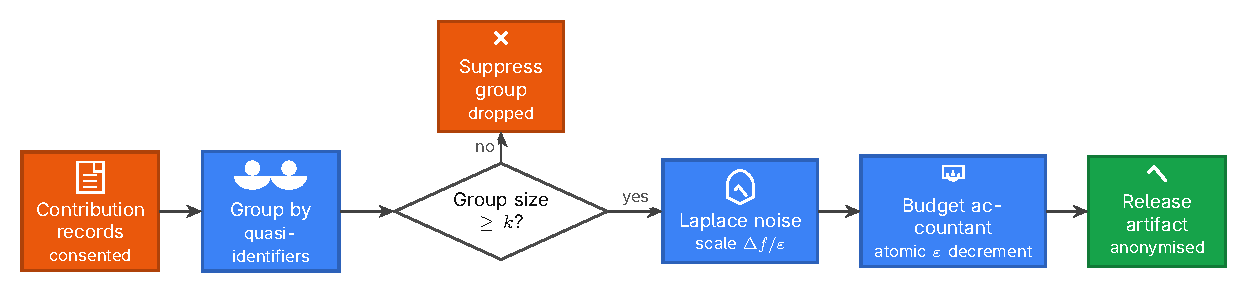
\includegraphics[width=\linewidth, totalheight=0.95\textheight, keepaspectratio]{../figures/schematics/fig-privacy-pipeline.pdf}
\caption{The privacy pipeline stages: records, grouping, k-anonymity, Laplace noise, and budget accounting.}
\label{fig:privacy-pipeline}
\end{figure}

\subsection{The EDC Connector Layer}

The design decision that shapes everything downstream is the choice to build the release boundary on a real IDSA-conformant connector rather than an application-level approximation of one. Eclipse Dataspace Components (EDC) provides the ODRL policy model, a policy engine with pluggable constraint functions, contract negotiation over the Dataspace Protocol, data plane and signaling infrastructure, and an event framework. It provides nothing for the offline-first device tier, the participant or steward interfaces, k-anonymity and differential privacy, or a participant-verifiable audit trail: those are the parts this project had to build itself, as the three connector extensions below and the TypeScript packages in section 3.3 describe.

EDC is pre-1.0 software with a roughly quarterly release cadence that has repeatedly shipped breaking changes. The reference implementation pins the connector to version 0.18.0 exactly and vendors the Gradle wrapper, recording the pin so that the manuscript's own reproducibility claims are attributable to a fixed dependency rather than a moving target. The 0.18.0 release alone changed the connector's default to data plane signaling, moved identity claims into the JWT \texttt{sub} claim, and replaced role-based authorization with scope-based authorization, any one of which would have silently invalidated an implementation written against the connector's documentation rather than its source. Identity in this deployment uses EDC's mock identity module (\texttt{org.eclipse.edc:iam-mock}) rather than IdentityHub with decentralized identifiers and verifiable credentials. Every claim this paper makes concerns what happens after a participant is already identified, so a full decentralized-identity stack was deliberately deferred rather than treated as a prerequisite, and this is stated here as a limitation rather than left implicit.

Registering a custom constraint function, binding it into the negotiation scope, and subscribing to connector events all had to be read from the 0.18.0 source directly rather than from documentation, because the release changed the shapes of exactly those APIs. Two further behaviors of the policy engine, discovered only by testing against a running connector rather than assumed from the design, are worth stating because they mark the implementation as real software rather than a paper design: EDC's management API rejects a policy definition outright, at creation time, if any of its constraints are bound to a scope but not to a registered function, so a compiler that emits a constraint ahead of the function that enforces it fails loudly rather than silently passing an unenforced rule. And the same API throws a \texttt{ClassCastException} on a numeric constraint right-operand, so the \texttt{consent-odrl} compiler in this implementation serializes every numeric threshold, including the steward-quorum count, as a string. Both are the kind of finding a specification cannot produce and only a build against the real connector can.

Three extensions realize the community-facing side of that connector. \texttt{benefits-policy} registers the BENEFITS-specific left operands the ODRL policy engine evaluates during contract negotiation, \texttt{PurposeFunction}, \texttt{RecipientClassFunction}, and \texttt{FieldSetFunction} for the consent-derived constraints, and \texttt{StewardQuorumFunction} for the release gate described in section 3.4. \texttt{benefits-privacy} implements the k-anonymity and differential-privacy pipeline described in section 3.5, exposed to the policy engine through its own \texttt{KAnonymityFunction} and \texttt{EpsilonBudgetFunction}. \texttt{benefits-audit} subscribes to the connector's event router and builds the Merkle-epoch audit chain described in section 3.6. This is a consolidation of the original design's four planned extensions, \texttt{benefits-policy}, \texttt{steward-quorum}, \texttt{privacy-pipeline}, and \texttt{audit-chain}, into three: the steward-quorum constraint function and its supporting store live inside \texttt{benefits-policy} alongside the other consent-derived constraint functions, rather than in a fourth, separate module.

Positioning this deployment against the closest comparators identified in the literature search is instructive about what "EDC in production" currently looks like elsewhere. \cite{mugge2023} implement a Catena-X connector, built on the same EDC family, for cross-company end-of-life-vehicle decision support, and validate it against a real cross-company data flow between named industrial roles. It is the strongest existing evidence that an EDC-based connector deployment can carry real, sovereignty-respecting data exchange for a concrete downstream use case rather than a synthetic demonstration, and this project's own community-connector deployment sits in the same thin but active empirical space. \cite{kalogeropoulos2023} integrate an IDS-connector-as-a-service into a Multi-access Edge Computing architecture and report scalability experiments, one of the few sources in this space with any quantitative evaluation, though at the edge-computing layer rather than at the connector's own policy-enforcement layer. \cite{norikane2025}, published in this paper's own target venue, model a data-space-based manufacturing supply chain and simulate its resilience under disruption. It evaluates supply-chain outcomes rather than connector-level properties, but it establishes that MDPI Systems already publishes verified, technically evaluated work on built data-space deployments, which is the venue precedent this chapter's own connector description follows.

\subsection{Paying for the Two-Language Boundary}

The choice to build the release boundary on a real connector has a direct cost: the connector is Java, and the device-tier consent filter has to run inside CouchDB's JavaScript validation engine, so the same consent semantics exist in two languages with no shared runtime between them. A single-language monorepo, considered and rejected during design, could have claimed one implementation of consent semantics shared by every enforcement point. The connector-based approach cannot make that claim, because the S1 evaluator at the device boundary and the S2 constraint functions at the connector boundary are necessarily separate code, written in separate languages, and free to drift apart without anyone noticing.

The consent model itself is designed once and compiled twice. \texttt{packages/consent-core} defines the rule model as a per-field grant of \texttt{(field, purpose, recipient class)}, its meet-semilattice composition operation (\texttt{meet.ts}, used when a released dataset draws on many participants whose grants differ, taking the narrowest purpose set, narrowest recipient class, intersection of fields, and earliest expiry across all of them), and the S1 evaluator itself (\texttt{evaluate.ts}). Two packages compile that single model into the system's two enforcement points: \texttt{consent-couchdb} bundles it into the CouchDB design document that becomes the \texttt{validate\_doc\_update} function running server-side inside CouchDB's own sealed query-server engine, and \texttt{consent-odrl} compiles it into the ODRL JSON-LD policy document that EDC's contract negotiation evaluates through the \texttt{benefits-policy} extension's constraint functions. TypeScript and Java exchange nothing but that JSON policy document. There is no shared library, shared type definitions, or remote procedure call between the two enforcement points, only an artifact both sides independently interpret.

That gap between two independent interpretations of the same document is exactly where drift becomes possible, and it is the one place in this design where a genuine engineering risk was accepted rather than designed away. The mitigation is a shared conformance-vector suite: a set of JSON test cases, each describing one grant configuration and one attempted access, that both the CouchDB validator and the connector's constraint functions must decide identically. The repository carries seventeen such vectors (\texttt{conformance/vectors}, covering cases such as a simple allowed access, a missing grant, an expired grant, a participant mismatch, and a purpose mismatch), each run against both implementations in their respective test suites, \texttt{ConformanceVectorTest} on the Java side and the corresponding suite in \texttt{consent-couchdb}'s own tests on the TypeScript side. The audit chain applies the identical strategy for its own two-sided risk, hashing computed on the connector side and re-verified on the participant side, with six further vectors (\texttt{conformance/audit-vectors}) exercised by \texttt{AuditConformanceVectorTest}. Table 1 lists all twenty-three vectors, the seventeen consent cases and the six audit cases, with the specific case each one exercises.

\begin{table}[H]
\caption{Consent and audit conformance vectors, with the specific case each one exercises.\label{tab:t1}}
\begin{tabularx}{\textwidth}{llX}
\toprule
Suite & Vector ID & What it tests \\
\midrule
Consent & v001-simple-allow & one field with an exactly matching unexpired grant \\
Consent & v002-missing-grant & a second field is present with no grant covering it \\
Consent & v003-expired-grant & the only grant for the field expired before now \\
Consent & v004-participant-mismatch & \texttt{consent.participantRef} differs from \texttt{record.participantRef} \\
Consent & v005-purpose-mismatch & \texttt{declaredPurpose} does not match the grant's purpose \\
Consent & v006-recipient-class-mismatch & \texttt{declaredRecipientClass} does not match the grant's recipient class \\
Consent & v007-not-a-contribution & type is not \texttt{contribution}, so S1 does not apply \\
Consent & v008-missing-consent & the \texttt{consent} property is absent from the record \\
Consent & v009-multi-field-ordering & several fields lack a covering grant. The alphabetically first one is reported \\
Consent & v010-expiry-exact-instant & a grant whose \texttt{expiresAt} equals now is expired (exclusive boundary) \\
Consent & v011-granted-at-exact-instant & a grant whose \texttt{grantedAt} equals now is active (inclusive boundary) \\
Consent & v012-null-grants & a \texttt{grants} value of null is treated as a missing consent assertion \\
Consent & v013-empty-grants & an empty \texttt{grants} array is present but grants nothing, so an uncovered field is reported \\
Consent & v014-malformed-fields & \texttt{fields} is a JSON array rather than the contracted object \\
Consent & v015-empty-string-grants & \texttt{consent.grants} is an empty string, neither absent nor null \\
Consent & v016-revoked-grant & a grant revoked before the record's evaluation instant is inactive \\
Consent & v017-revocation-not-yet-effective & a revocation timestamped after the evaluation instant has not taken effect yet \\
Audit & av001-single-leaf & a single-entry tree. The root is that entry's own leaf hash \\
Audit & av002-two-leaves & an even-sized tree, one pairing, no promotion \\
Audit & av003-three-leaves-odd-promotion & an odd-sized tree. The third leaf is promoted unhashed to the second level \\
Audit & av004-five-leaves & a larger odd-sized tree spanning two levels of promotion \\
Audit & av005-separator-in-plain-language & a field value containing the raw separator character, escaped identically in both languages \\
Audit & av006-backslash-in-actor & a field value containing a raw backslash, escaped identically in both languages \\
\bottomrule
\end{tabularx}
\end{table}

This converts a structural weakness into a publishable artifact rather than merely patching around it. As the design record for this project puts it, releasing a set of conformance vectors and demonstrating that edge and connector enforcement agree on all of them is a stronger correctness claim than asserting the code was written once, because the claim survives exactly the failure mode a single shared implementation cannot even expose: two independent implementations reaching the same decision on every case that matters, not by construction, but by test.

Both of the enforcement points just described, the S1 evaluator at the device boundary and the S2 constraint functions at the connector boundary, gate writes: whether a record may leave the device and whether a release may be negotiated. Neither, as originally built, gated whether an already-written contribution could be included in a query-time aggregate: \texttt{Contribution}, the record type \texttt{benefits-privacy}'s \texttt{PrivacyPipeline} and \texttt{KAnonymity} actually operate on, carried no consent information at all, so an aggregate query result could include a contribution regardless of the consent scope its owner had actually granted, once that contribution had already been written. This gap went unaddressed until the G2 experiment (Chapter 5, Chapter 6) required closing it. Doing so meant building query-time consent scoping into \texttt{PrivacyPipeline} itself, wiring a new \texttt{ConsentGrant} type and a query-purpose-and-recipient-class filter into the production pipeline rather than into the experiment harness alone, so this is a real, additive production capability this project added, not a test fixture confined to G2.

\subsection{The Steward-Quorum Release Gate}

SIDS 2026's own description of the steward gate was explicit and specific: aggregated outputs wrapped in a cryptographic envelope keyed by steward quorum, with the decryption key released only on receipt of a co-signed authorization token, and the reference-implementation design that followed it retained Shamir secret sharing over the payload content key as, in its own framing, a second lock on release, because a policy engine the operator runs is not the same guarantee as cryptographic impossibility, and that difference is exactly what a skeptical reviewer would press on.

That cryptographic second lock was not carried into the built system. The \texttt{benefits-policy} extension's \texttt{StewardAuthorization} record holds a release request identifier, a dataset hash binding the token to an exact dataset, a list of steward signatures, and separate lists of reviews, vetoes, and appeals. It carries no key shares, and no component of \texttt{benefits-privacy}'s \texttt{ReleaseArtifact} store encrypts its bytes under a quorum-reconstructed key. What is actually enforced is a signature-count threshold: \texttt{StewardQuorumFunction}, registered as an ODRL constraint function and evaluated during contract negotiation, reads the release request identifier from a sibling constraint on the same permission (EDC's policy context carries no general-purpose data map, so the quorum function locates its state this way rather than off the evaluation context directly), looks up the corresponding \texttt{StewardAuthorization}, counts the number of distinct stewards who have signed it, and refuses the negotiation unless that count meets or exceeds the threshold the policy names. Contract negotiation cannot complete without that quorum, so the gate is real and release-blocking, but the mechanism realizing it is a policy-engine check against a database-backed authorization record, not a cryptographic envelope that makes unauthorized release mathematically impossible regardless of who operates the connector. This is a narrower guarantee than SIDS 2026 described and than the design specification that followed it originally called for, and the manuscript states that gap here rather than silently rewriting the earlier claim to match what was built.

A second gap, more serious than the cryptographic one just stated, sits alongside it. SIDS 2026's own text specifies a veto, not merely a quorum, as part of the steward gate: "for each release, two of three rotating stewards must co-sign an authorization token; any single steward may veto, in which case the release request is returned to the requester with a written justification" \cite{katrakazas2026}. The built system does not enforce this. \texttt{StewardQuorumFunction.evaluate} reads only \texttt{authorization.distinctStewardCount() >= required}. It never reads \texttt{authorization.vetoes()}, confirmed directly in the source. A steward can record a veto today, through the same \texttt{StewardAuthorization} record that already carries a \texttt{vetoes} list alongside its signatures, reviews, and appeals, but that recorded veto has no effect on whether contract negotiation succeeds: a release with a satisfied signature count clears the gate whether or not a steward has vetoed it. It is the predecessor paper's own specified policy, published before this system was built, and the built system silently does not enforce it. Unlike the cryptographic-envelope gap, which diverges from an internal design intent that a reference implementation stopped short of realizing, this gap diverges from a guarantee SIDS 2026 explicitly promised its readers, which is why it is treated here as the more serious of the two.

That gap changes how this mechanism should be read against its closest technical comparators. \cite{kokoriskogias2020} describe CALYPSO, in which confidential "on-chain secrets" require an actual threshold of a trustee committee to decrypt, benchmarked directly against committee size, with latency scaling from roughly 0.2 to 8 seconds as the committee grows from 16 to 128 members. Release there is gated by genuine threshold decryption, so no subset of the committee smaller than the threshold can produce the plaintext under any circumstance. \cite{raisaro2019} describe MedCo, a deployed clinical and genomic data-sharing system in which decrypting pooled query results requires the collective participation of every federated site holding a key share, again a real distributed-decryption gate rather than a policy check. Both are stronger comparators in the cryptographic sense than a contrast: they hold the property the original BENEFITS design aspired to and the built system does not yet realize. What this implementation does hold in common with them is the auditable, quorum-of-independent-parties structure around the release decision: signature, review, veto, and appeal records are all held alongside one another in \texttt{StewardAuthorization}, and the framing that a single actor should never unilaterally control disclosure. What it does not yet hold is CALYPSO's and MedCo's cryptographic independence from the operator of the software making the check, and, per the veto gap stated above, the recorded vetoes it does hold are not yet consulted by the release decision itself. A veto is recorded, not enforced. Stating this precisely, rather than describing the built gate as equivalent to threshold decryption, is itself part of what this chapter reports about the system as it currently stands.

\subsection{The Privacy Pipeline}

The \texttt{benefits-privacy} extension implements the anonymization stage SIDS 2026 described as an architectural primitive rather than a compliance afterthought. \texttt{KAnonymity} computes the structural k of a candidate release and \texttt{KAnonymityFunction} exposes that computation to the policy engine as an ODRL constraint, so a release whose computed k falls below the policy's threshold is refused at contract negotiation rather than filtered after the fact. \texttt{LaplaceNoiseSource}, sitting behind the shared \texttt{NoiseSource} interface, adds calibrated Laplace noise to statistical query results, and \texttt{BudgetAccountant} (with \texttt{InMemoryBudgetAccountant} and \texttt{CouchDbBudgetAccountant} implementations) tracks cumulative privacy loss against a per-site budget, exposed to the policy engine through \texttt{EpsilonBudgetFunction} so that a query exceeding the remaining allowance is refused the same way an under-threshold k value is. \texttt{PrivacyPipeline} composes k-anonymity, noise addition, and budget accounting into the sequence a release request actually passes through, and \texttt{ReleaseArtifact} stores the computed result once rather than recomputing it per transfer, a deliberate choice: recomputing per transfer would let a requester repeat the same transfer and average results to recover the true value while the budget accountant had charged epsilon only once, defeating the accounting it exists to enforce.

Two of these constraint functions did not exist when the connector's policy compiler was first written, and the design specification is explicit that this was tested against a running connector rather than assumed: EDC rejects an entire policy document at creation time if it names a constraint bound to no registered function, so \texttt{consent-odrl} could not emit \texttt{benefits:kAnonymity} or \texttt{benefits:epsilonBudget} constraints until \texttt{KAnonymityFunction} and \texttt{EpsilonBudgetFunction} existed to enforce them, and the compiler's options for those two constraints were removed from its interface entirely in the interim rather than left present but silently unenforced, on the reasoning that an option a caller can set while nothing checks it is a false affordance worse than no option at all.

This pipeline sits between two identifiable lines of prior work. \cite{mironov2017} supplies the theoretical grounding much of the modern budget-accounting literature is built on, Rényi differential privacy, a relaxation that generalizes and recovers the moments-accountant approach as a special case and admits substantially tighter composition than naive sequential composition, and the accounting discipline behind \texttt{BudgetAccountant}'s cumulative-loss tracking descends from that same lineage even though the pipeline itself uses simple Laplace mechanisms rather than an RDP-based accountant specifically. \cite{prasser2020} describe ARX, an actively maintained, real anonymization tool that combines k-anonymity and related structural models with a differential-privacy mode and built-in utility metrics, the closest existing tool that pairs structural anonymization and formal DP the way this pipeline's \texttt{KAnonymity} stage and \texttt{LaplaceNoiseSource} stage are paired here. Where ARX is a general-purpose, standalone anonymization tool applied after the fact to a dataset, \texttt{benefits-privacy}'s pipeline is embedded directly in the connector's contract-negotiation path, so a release that would violate either bound is refused before data leaves the boundary rather than flagged by a separate tool a step later.

\subsection{The Audit Chain}

\texttt{benefits-audit} implements the tamper-evident record SIDS 2026 described as hash-chained, but batches entries into epochs rather than chaining every entry directly, on a specific design rationale: a pure hash chain forces a verifying participant to hold every entry in the log to check their own, which leaks the existence and timing of other participants' access events to anyone checking their own record. Instead, \texttt{MerkleTree} builds a Merkle tree over the entries within one epoch, \texttt{EpochSealer} seals that epoch by committing its root, and \texttt{AuditHashing} chains only the epoch roots to one another, so a participant can obtain their own entries, an inclusion proof for each, and the root chain, proving their entries are present and unaltered while learning nothing about anyone else's. \texttt{BenefitsAuditEventListener} subscribes to the connector's \texttt{EventRouter} and is the component intended to make the log a record of what the connector actually did rather than something an application component writes about itself. \texttt{AuditStore}, with \texttt{InMemoryAuditStore} and \texttt{CouchDbAuditStore} implementations, persists the resulting entries and epochs, and the paired TypeScript package \texttt{audit-verify} (\texttt{chain.ts}, \texttt{hashing.ts}, \texttt{merkle.ts}) implements the participant-side half of the same verification, so that inclusion and consistency checks do not depend on trusting the connector that produced them.

The claim that the log records "every negotiation, policy decision, and transfer" was written before any EDC event had ever been observed firing, and testing it against a running connector overturned part of it. A negotiation offer refused because it fails ODRL constraint evaluation, whether for missing steward quorum, purpose mismatch, recipient-class mismatch, an out-of-grant field, an expired grant, insufficient k, or an exhausted privacy budget, is rejected by EDC 0.18.0 synchronously, inside its Dataspace Protocol handler, before any \texttt{ContractNegotiation} entity is created. Because EDC's event system fires only from state-machine transitions on entities that exist, and no entity is created for this class of refusal, no event is ever published for it. This was confirmed empirically by forcing a real policy-refused negotiation against a running provider and observing a 400 response paired with zero corresponding lines in the provider's own event log. The audit chain therefore does not cover the conformance suite's refusal cases specifically, precisely the "policy decision" the steward-quorum, k-anonymity, and epsilon-budget machinery exists to make. What it does cover is every negotiation admitted into the provider's state machine, whether it later succeeds or is terminated, and every transfer attempt. A cheaper fix, having a constraint function record its own refusal into the log the moment it returns false, was considered and rejected, because it would restore coverage only by having the log contain entries an application component chose to self-report, exactly where independent, connector-native proof matters most. This boundary, not the original "every policy decision" phrasing, is what this paper claims about the audit chain's coverage.

Positioned against prior art, the mechanism descends directly from \cite{schneier1999}, whose scheme couples chained one-way hashes, which establish the retroactive-tamper-detection guarantee that any alteration of an already-hashed entry breaks the chain from that point forward, with forward-secure MACs, which are what make entries written before a compromise unreadable to an attacker who later controls the logging machine. SIDS 2026's own architecture section invokes the tamper-detection half of this guarantee without tracing it to a source. The epoch structure itself follows the real-world deployed precedent of Certificate Transparency \cite{laurie2013}, which defines standardized Merkle audit paths and consistency proofs for publicly logging TLS certificate issuance and has run at internet scale since its 2013 publication as RFC 6962, later superseded by RFC 9162 (Certificate Transparency Version 2.0). Major browsers required Certificate Transparency for TLS certificates for several years following its deployment. Where Certificate Transparency's epochs are global and its proofs are about certificate issuance visible to any observer, this system's epochs are sealed periodically over participant contribution events and its inclusion proofs are scoped so a participant learns only about their own entries, the privacy property the pure hash-chain alternative could not offer.

\subsection{What the Phase Gates Verified}

The build proceeded through eight gated phases, each required to pass before the next began, because the correctness claims in this design are the contribution and needed to be test-first rather than retrofitted. What the gates actually established, rather than what was merely planned, is the honest summary of what this chapter can claim as built. The skeleton phase established that the pinned connector's Management API answers, that CouchDB is reachable, and that a custom constraint function can be observed evaluating during a real two-connector negotiation, with the CouchDB query server's engine probed and recorded rather than assumed. The consent-core phase established that the conformance vectors pass and that a real CouchDB instance, running the compiled validation function, rejects an unconsented write. The policy and steward-quorum phase established that the consent-derived conformance cases pass and that contract negotiation is refused without a satisfied steward quorum, against a running connector rather than a mock. Table 2 lists all nine cases this phase's gate checked, each a real contract negotiation against the connector rather than a unit test. All nine passed.

\begin{table}[H]
\caption{Enforcement-correctness cases checked at the policy and steward-quorum gate. All nine passed.\label{tab:t2}}
\begin{tabularx}{\textwidth}{lllX}
\toprule
Case & Expected & Observed & Discriminating evidence \\
\midrule
quorum-met & FINALIZED & FINALIZED & signed=2, required=2 \\
quorum-missing & TERMINATED & TERMINATED & no steward authorization seeded for the request \\
quorum-one-steward-twice & TERMINATED & TERMINATED & two signatures from one steward counted as signed=1 \\
purpose-mismatch & TERMINATED & TERMINATED & requester purpose \texttt{marketing} against policy purpose \texttt{service-improvement} \\
recipient-class-mismatch & TERMINATED & TERMINATED & requester recipient class \texttt{provider} against policy \texttt{statistics} \\
field-outside-grant & TERMINATED & TERMINATED & requested \texttt{health.condition} outside granted \texttt{service.satisfaction} \\
expired-grant-field-excluded & TERMINATED & TERMINATED & expired \texttt{health.condition} grant excluded from the compiled policy \\
k-below-threshold* & TERMINATED & TERMINATED & \texttt{computedK}=4 below \texttt{required}=5 \\
budget-exceeded* & TERMINATED & TERMINATED & \texttt{charged}=0.9 above \texttt{cap}=0.5 \\
\bottomrule
\end{tabularx}
\end{table}

The two cases marked with an asterisk exercise \texttt{KAnonymityFunction} and \texttt{EpsilonBudgetFunction} against a directly-seeded \texttt{ReleaseArtifact} rather than one produced by a live \texttt{PrivacyPipeline} run. The artifact's \texttt{computedK} and \texttt{epsilonCharged} are seeded values chosen to land on each side of the policy threshold, not values the pipeline itself computed from real contributions. \texttt{PrivacyPipeline.compute} is proven separately, end to end, by \texttt{PrivacyPipelineTest}, \texttt{KAnonymityTest}, \texttt{LaplaceNoiseSourceTest}, and \texttt{InMemoryBudgetAccountantTest}.

The audit-chain phase established that mutated entries, mutated roots, and reordered epochs are each detected at the mechanism level in every case tested, with the formal proof-size and verification-time sweep against epoch size deferred to the later experiment phase rather than folded into this gate. The device-fleet phase and the interface phase built the simulated PouchDB fleet used for the revocation-under-partition experiment and manually click-tested the participant-web and steward-portal applications, producing the screenshots this manuscript can draw on. That fleet's revocation mechanism is a client-side purge, not a server-side re-check: \texttt{Device.revoke} mutates the device's own local grant state and, in the same call, removes any not-yet-synced contribution record matching the revoked field, purpose, and recipient class from the device's local queue, before that record is ever replicated to CouchDB. The CouchDB \texttt{validate\_doc\_update} function does not provide an independent second check of this: it evaluates a contribution record's own embedded \texttt{consent.grants} snapshot, taken at write time, against the live server clock, but it has no access to the device's current grant state and so cannot detect that a grant embedded in an already-queued record has since been revoked. A queued record the device failed to purge before syncing would still pass that validation on its stale, embedded consent. E2's zero-leaked-record result (section 5.2) therefore verifies that the device-side purge works on every tested duty cycle, not that the server independently catches what the device failed to withhold.

Taken together, these gates are the evidentiary basis for the claim this chapter opened with: the architecture SIDS 2026 sketched is now real, running software, not a specification awaiting pilot deployment. That software is not identical to the design that preceded it. The steward-release gate is a policy-engine check backed by a signature quorum rather than the cryptographic envelope originally proposed, that same gate does not enforce the single-steward veto SIDS 2026 specified even though it records vetoes, and the audit chain's coverage stops at the boundary of policy-refused negotiations rather than extending to every policy decision as first written. Reporting all three corrections plainly, alongside what the gates did establish, is what distinguishes this chapter's account of the system from the specification it replaces.
